\documentclass[a4paper,11pt]{article}
  % Métadonnées
  \title{Analyse d'article\\\large Adaptation continue en environnement non stationnaire et compétitif via méta-apprentissage}
  \author{Lecoq Simon (LECS09129600)}
  \date{}
  \usepackage{graphicx}
  \usepackage[lofdepth,lotdepth]{subfig}
  \usepackage{float}
  \begin{document}
    % Titre
    \maketitle
  
    % Style
    \setlength{\parindent}{0ex}
    \setlength{\parskip}{1em}

    % Introduction
    \section{Introduction}
    L’article discuté ici a été présenté lors de l’ICLR 2018 
    \textit{(International Conference on Learning Representations)} et s’intitule 
    \textit{Continious Adapatation via Meta-Learning in Nonstationary and Competitive 
    Environments}\textsuperscript{\cite{paper}}.

    Les auteurs présentent rapidement les accomplissements réalisés grâce aux progrès dans 
    l’apprentissage par renforcement (maîtriser les jeux de l’Atari 2600, vaincre des champions
    du Go, IA conversationnel, …) mais soulignent que la majorité des algorithmes utilisés 
    supposent un environnement stationnaire.

    Les difficultés de l’apprentissage en environnement non stationnaire sont mises 
    en évidence : complexité, aspects continu et évolutif, diverge des données d'apprentissage. 
    Les approches actuelles pour pallier le problème sont mentionnées : détection de contexte ou 
    suivi d’événements (tracking). Les auteurs expliquent cependant 
    que ces méthodes ne sont pas adaptées pour un fonctionnement en \textit{"few-shot regime"}. 
    
    Le papier cherche à répondre aux problématiques de l'apprentissage en environnement non 
    stationnaire grâce à l'adaptation continue et du méta-apprentissage.

    L'approche proposée ici est de considérer l'environnement non stationnaire comme une 
    séquence de tâches stationnaires afin de pouvoir la représenter par une chaîne de Markov. 
    Une version altérée du modèle agnostique de méta-apprentissage MAML (Finn et al., 2017b) sera 
    utilisée, et deux environnements avec physique simulée ont été mis en place dans l'optique de 
    tester l'adaptation continue.


    % Prérequis
    \section{Prérequis}

    \subsection{Environnement non stationnaire}
    \vspace{-1em}
    Environnement où un changement radical du fonctionnement de celui-ci peut se produire. 
    La non stationnarité peut par exemple être induite par l’apprentissage de chaque 
    agent dans un environnement multi-agent.

    \subsection{Méta-apprentissage}
    \vspace{-1em}
    Consiste à produire des règles d’apprentissage flexibles qui 
    peuvent être appliquées quel que soit la situation. Ainsi, en cas de changement du monde 
    dans lequel un agent évolue, celui-ci sera capable de produire un résultat satisfaisant 
    rapidement à partir d’un entrainement très limité.

    \subsection{Adaptation continue}
    \vspace{-1em}
    Consiste à réussir à opérer dans une unique tâche dans un environnement non stationnaire 
    en s’adaptant aux changements de celui-ci à l’exécution et avec des jeux de données ou un 
    nombre d’interactions limité avant que l’environnement ne change de nouveau.

    % Proposition
    \section{Proposition}

    % Présentation des travaux
    \subsection{Présentation des travaux}
    \vspace{-1em}

    Les auteurs ont basé leur travaux sur le MAML (Finn et al., 2017b) et l'ont étendu 
    avec une vision probabiliste du monde.
    \begin{equation}
      \Phi := \theta - \alpha\nabla_\theta L_T(\tau_\theta^{1:K})
    \end{equation}

    L'objectif du méta-apprentissage est de produire à l'aide d'une expérience 
    limitée une politique efficace $\Phi$ permettant d'accomplir une tâche $T$ prélevée 
    d'une distribution $D(T)$. 
    
    Après avoir récupéré $K$ trajectoires $\tau_\theta$ sous l'ancienne politique $\theta$, 
    une nouvelle politique $\Phi$ est construite en essayant de minimiser la perte $L_T$ de $T$ via son gradient.
  
    Aucune hypothèse n'est normalement faite sur $D(T)$, mais étant donné qu'ici l'environnement
    est vu comme une chaîne de Markov, $D(T)$ est défini par les évolutions de celui-ci et 
    les tâches sont séquentiellement dépendantes entre elles. Cette propriété permet de définir 
    la méta-perte $L_{T_i, T_{i+1}}$ entre deux tâches consécutives $T_i$, $T_{i+1}$ afin de calculer 
    le coefficient d'adaptation $\alpha$. 
    
    % Expérimentation
    \subsection{Expérimentation}
    \vspace{-1em}

    % Figures sur l'expérimentation
    \begin{figure}[h]
      \centering
      \subfloat[]{\label{fig:about-a}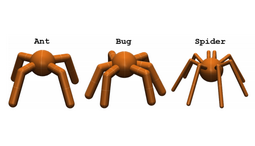
\includegraphics[width=0.3\textwidth]{fig1a.png}}
      \subfloat[]{\label{fig:about-b}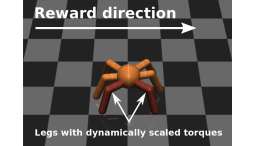
\includegraphics[width=0.3\textwidth]{fig1b.png}}
      \subfloat[]{\label{fig:about-c}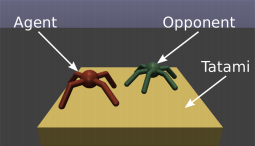
\includegraphics[width=0.3\textwidth]{fig1c.png}}
      \caption{(a) Morphologies des agents, (b) exercice 1, (c) exercice 2.}
      \label{about}
    \end{figure}

    Les deux exercices suivants ont été soumis à des agents de différentes morphologies (fig. \ref{about}a), 
    politiques et méthodes d'adaptation :  

    \begin{enumerate}
      \vspace{-0.5em}
      \item{
        Se déplacer rapidement dans une direction fixée (fig. \ref{about}b). 
        À chaque épisode, deux membres de l'agent sont progressivement paralysés. 
      }
      \item{
        Un jeu où deux agents tentent de renverser leur adversaire ou de le faire sortir du ring (fig. \ref{about}c). 
        Chaque partie contient plusieurs manches et l'agent est autorisé à mettre à jour sa politique. Le jeu a été équilibré au préalable de façon à ce 
        que chaque type d'agent ait les mêmes chances de gagner.
      }
      \vspace{-0.5em}
    \end{enumerate}

    L'objectif est d'évaluer l'efficacité de différentes méthodes d'adaptation : 
    aucune, implicite (avec $RL^2$), tracking (PPO) et méta-apprentissage. Pour éviter les biais, 
    des mesures spécifiques ont étés mises en place et les 3 types de politiques suivantes ont été 
    utilisés : Perceptron multicouche (MLP), Réseau récurrent (LSTM) et $RL^2$.
    
    % Résultats
    \section{Résultats}

    Pour le premier exercice (fig. \ref{ex1}), on constate que les politiques utilisant le méta-apprentissage sont 
    sous-optimales par rapport aux autres méthodes lors du premier épisode, mais qu'après deux ou trois 
    épisodes les performances sont similaires, et à l'issue des sept épisodes, elles sont nettement meilleures.
    On constate que le tracking n'améliore pas significativement les résultats par rapport à une politique sans adaptation, 
    et les performances sont même parfois inférieures.

    En ce qui concerne le second exercice (fig. \ref{ex2}) qui introduit une dimension compétitive, plusieurs remarques 
    peuvent être faites. Les réseaux récurrents sont les plus efficaces, par leur capacité à garder en mémoire les épisodes récents.
    Les politiques avec une adaptation par méta-apprentissage sont systématiquement classés parmi les plus performants. 
    Une étude portée sur l'évolution de 1050 agents a aussi été réalisée, dans laquelle les perdants été supprimés et les vainqueurs dupliqués. 
    Au bout de 10 générations, les agents avec méta-apprentissage constituaient près de 85\% de la population. 
    
    % Figure résultats déplacement
    \begin{figure}[h]
      \centering
      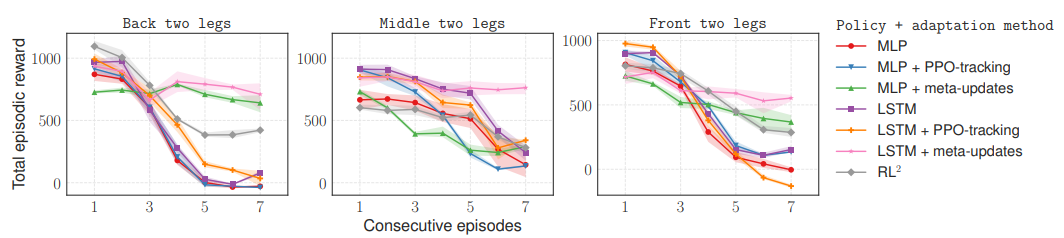
\includegraphics[width=\textwidth]{fig2.png}
      \caption{(exercice 1) : Récompenses sur 7 épisodes consécutifs des agents avec différentes politiques et méthodes d'adaptations.}
      \label{ex1}
    \end{figure}

    % Figure résultats compétition
    \begin{figure}[h]
      \centering
      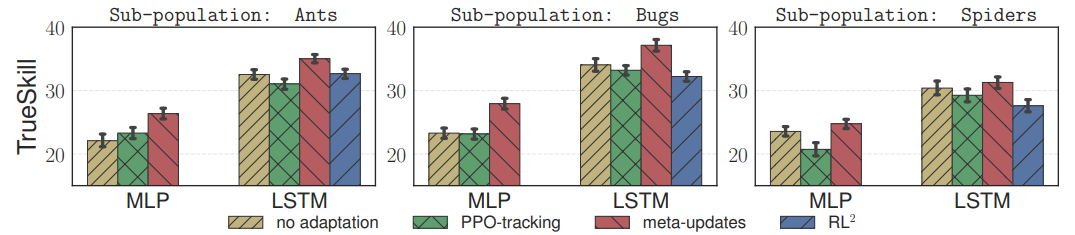
\includegraphics[width=\textwidth]{fig3.png}
      \caption{(exercice 2) : Classement TrueSkill par performance des agents utilisant un MLP ou un LSTM dans une population de 105 agents pré-entrainés après 1000 parties.}
      \label{ex2}
    \end{figure}

    % Discussion
    \section{Discussion}

    Les auteurs proposent donc une solution intéressante pour offrir un apprentissage efficace 
    dans un environnement non stationnaire par l'intermédiaire de l'adaptation continue.

    Un des points discutés dans l'article étudié est la performance de chaque méthode d'adaptation 
    selon le nombre d'épisodes à disposition. Le méta-apprentissage est très performant lorsque peu 
    d'expérience est à disposition, mais semble ne pas pouvoir améliorer son efficacité quand de nouvelles 
    données sont disponibles tandis que le tracking peut quasiment réaliser un apprentissage à la volée\textsuperscript{\cite{paper}}.
    
    Il serait donc intéressant de déterminer la cause de la stagnation des performances du méta-apprentissage.
    Avec le modèle actuel, si l'environnement non stationnaire n'est pas particulièrement instable, 
    le tracking\textsuperscript{\cite{sutton}} semble produire de meilleurs résultats sur le long terme.

    L'aspect coopératif des environnements compétitifs (e.g. combats en équipe) n'est pas abordé et 
    pourrait être étudié dans de futurs travaux, afin d'y évaluer les performances de l'adaptation 
    continue. Il serait intéressant de les comparer aux IA de DeepMind conçues pour la capture de drapeau sur 
    le jeu Quake 3\textsuperscript{\cite{jaderberg}} ou même plus généralement pour résoudre des problèmes multi-agents qui ne 
    sont pas uniquement compétitifs\textsuperscript{\cite{raluca}}.

    % Conclusion
    \section{Conclusion}

    L'adaptation continue par méta-apprentissage est ici discutée pour répondre aux problématiques de l'apprentissage
    en environnement non stationnaire. Les résultats des deux expérimentations réalisées ont démontré
    des résultats convaincants et suggèrent que le modèle est viable et exploitable.

    Toutefois, les performances semblent être plafonnées avec le modèle actuel et ne semble donc pas 
    pouvoir être utilisé en toute circonstances. Des travaux futurs pourraient étudier la question de 
    la coopération entre plusieurs agents utilisant l'adaptation continue.

    % Références
    \begin{thebibliography}{9}
      \bibitem{paper}
        Maruan Al-Shedivat, Trapit Bansal, Yura Burda, Ilya Sutskever, Igor Mordatch et Pieter Abbeel.
        \emph{Continious Adapatation via Meta-Learning in Nonstationary and Competitive Environments}.
        2018
      \bibitem{sutton}
        Richard S Sutton, David A McAllester, Satinder P Singh, and Yishay Mansour.
        \emph{Policy gradient methods for reinforcement learning with function approximation}.
        In Advances in neural information processing systems, pp. 1057–1063, 2000.
      \bibitem{raluca}
        Raluca D. Gaina, Adrien Couetoux, Dennis J.N.J. Soemers, Mark H.M. Winands, Tom Vodopivec, ..., Diego Perez-Liebana.
        \emph{The 2016 Two-Player GVGAI Competition}
        2017
      \bibitem{jaderberg}
         Max Jaderberg, Wojciech M. Czarnecki, Iain Dunning, Luke Marris, Guy Lever, ..., Thore Graepel.
        \emph{Human-level performance in first-person multiplayer games with population-based deep reinforcement learning}
        2017
    \end{thebibliography}
 
  \end{document}



